\section*{Lecture 23}

\subsection*{1.} Consider the surface $S$ consisting of all points $P(x,y,z)$ such that
\[ 
y + z = c
.\]

\paragraph{(a)} Sketch the surface $S$ for $c=0$. Calculate the unit normal vector. Sketch some of the unit surface normal vectors.
\begin{figure} [ht]
  \centering
  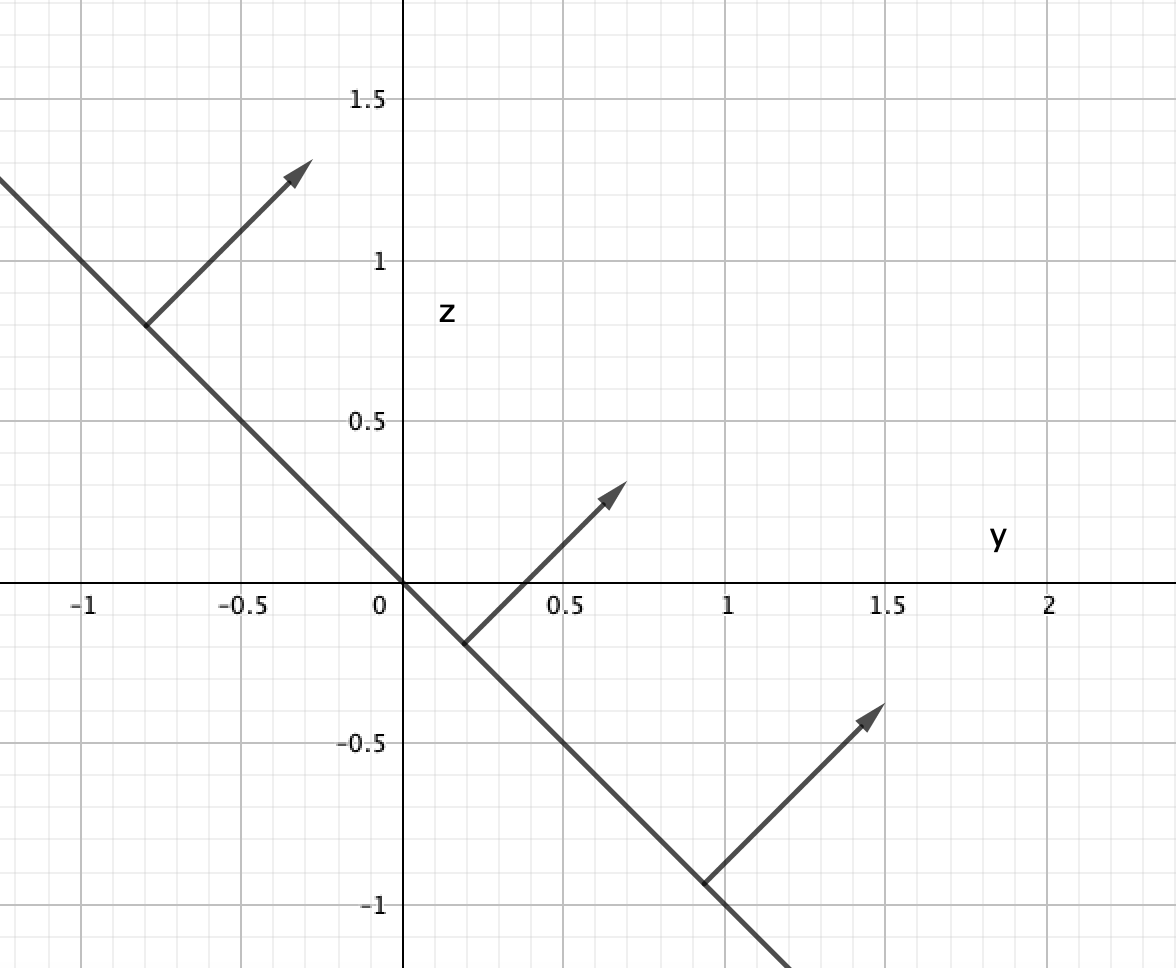
\includegraphics[width=0.5\linewidth]{./figures/e23f1.png}
  \caption{Surface $S = 0$}
  \label{fig:e23f1}
\end{figure}
The gradient can quickly be seen to be:
\[ 
\nabla f (x,y,z) = \left( 0,1,1 \right) 
.\]
Which gives the unit surface normal vector of:
\[ 
\Vec{n}\left( x,y,z \right) = \frac{\nabla f \left( x,y,z \right) }{\left| \nabla f \left( x,y,z \right)  \right|} = \frac{\left( 0,1,1 \right) }{\sqrt{2}} = \left( 0, \frac{1}{\sqrt{2}}, \frac{1}{\sqrt{2}} \right) 
.\]


\paragraph{(b)} Sketch the surface $S$ for $c = 1$. Calculate the unit normal vector. Sketch some of the unit normal vectors.
\begin{figure} [ht]
  \centering
  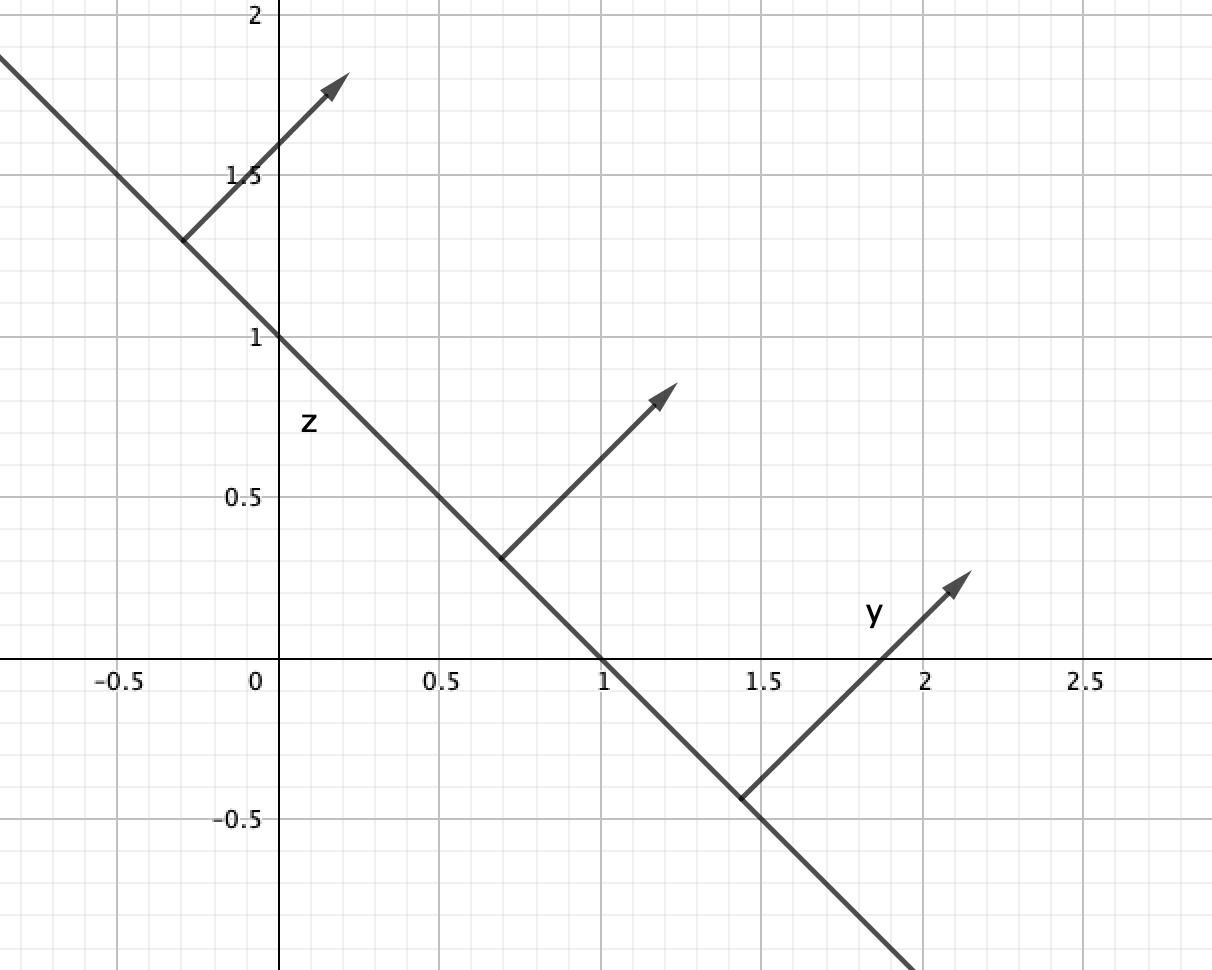
\includegraphics[width=0.5\linewidth]{./figures/e23f2.png}
  \caption{Surface $S = 1$}
  \label{fig:e23f2}
\end{figure}
The gradient and therefore the unit normal vectors are the same here. 

\subsection*{2.} Consider the surface $S$ consisting of all points $P(x,y,z)$ such that
\[ 
x^2 + y^2 = 1, \qquad x > 0, \qquad y > 0, 0 \leq z \leq 1
.\]
Sketch the surface $S$. Calculate the unit surface normal vector. Sketch some of the unit surface normal vectors.
\begin{figure} [ht]
  \centering
  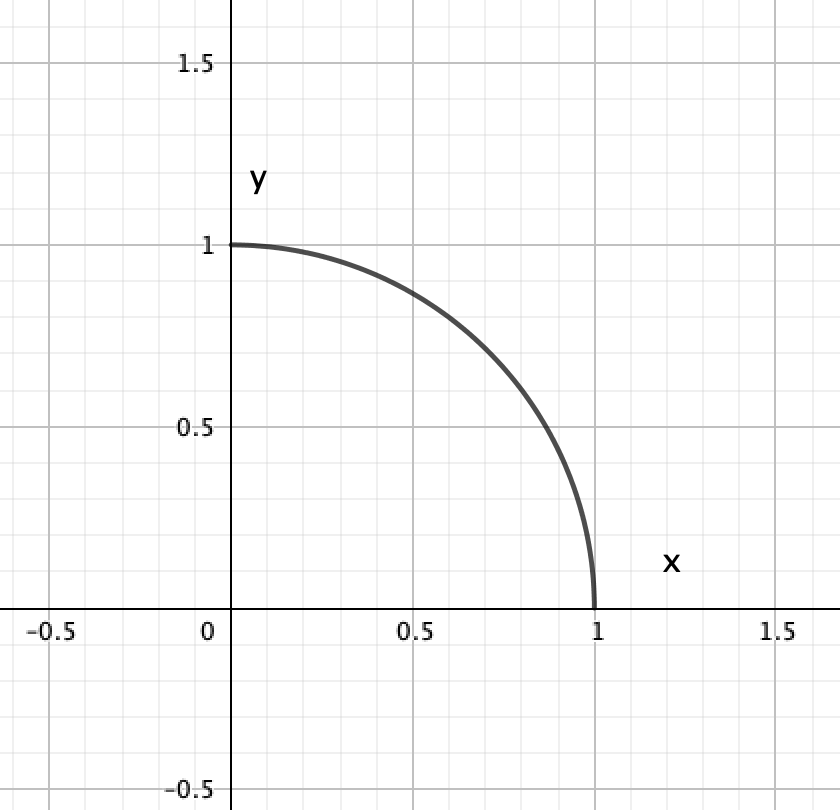
\includegraphics[width=0.5\linewidth]{./figures/e23f3.png}
  \caption{Surface $x^2 + y^2 = 1$}
  \label{fig:e23f3}
\end{figure}
Here the gradient is:
\[ 
\nabla f \left( x,y,z \right) = \left( 2x, 2y, 0 \right) 
.\]
And the unit normal vector is therefore:
\[
  \Vec{n}\left( x,y,z \right) = \frac{\nabla f \left( x,y,z \right) }{\left| \nabla f \left( x,y,z \right)  \right|} = \frac{\left( 2x,2y,0 \right) }{\sqrt{4x^2 + 4y^2}} = \frac{\left( 2x, 2y, 0 \right) }{2 \sqrt{x^2 + y^2}} = \left( x,y, 0 \right) 
.\]



\subsection*{3.} Calculate the directional derivative of

\paragraph{(a)} $f(x,y,z)=xyz$ at $P(1,1,1)$ in direction $\Vec{b} = \left( 1,1,1 \right) $
\bigbreak
First the gradient is found to be:
\[ 
\nabla f \left( x,y,z \right) = \left( yz, xz, xy \right) 
.\]
This gives a gradient at $P$ of:
\[ 
\nabla f \left( 1,1,1 \right) = \left( 1,1,1 \right) 
.\]
The directional derivative can therefore be found as:
\[ 
D_{\Vec{b}}\left( P \right) = \frac{\nabla f(P) \cdot \Vec{b}}{\left| \Vec{b} \right|} = \frac{\left( 1,1,1 \right) \cdot \left( 1,1,1 \right) }{\sqrt{1^2+1^2+1^2}} = \frac{3}{\sqrt{3}} = \sqrt{3}
.\]



\paragraph{(b)} $f(x,y,z)= \cos \left( xyz \right) $ at $P(1, \frac{\pi}{2}, 1)$ in direction $\Vec{b} = \left( 1,1,1 \right) $
\bigbreak
Here the gradient is:
\[ 
\nabla f \left( x,y,z \right) = \left( - yz \sin \left( xyz \right), - xz \sin \left( xyz \right) , - xy \sin \left( xyz \right)  \right) 
.\]
This gives a gradient at $P$ of:
\[ 
\nabla f(P) = \left( - \frac{\pi}{2}, -1, - \frac{\pi}{2} \right) 
.\]
The directional derivative can therefore be found as:
\[ 
D_{\Vec{b}}(P) = \frac{\nabla f (P) \cdot \Vec{b}}{\left| \Vec{b} \right|} = \frac{ \left(- \frac{\pi}{2}, -1, - \frac{\pi}{2} \right) \cdot \left( 1,1,1 \right) }{\sqrt{3}} = \frac{-\pi - 1}{\sqrt{3}}
.\]



\subsection*{4.} Calculate the divergence of

\paragraph{(a)}
\[ 
\Vec{v} \left( x,y,z \right) = \left( x^{y}, yz, \left( xy + zx \right)^3 \right) 
.\]
\bigbreak
Here we get:
\[ 
\nabla \cdot  \Vec{v} \left( x,y,z \right) = y x^{y-1} + z + 3 \left( xy + zx \right)^2 x
.\]


\paragraph{(b)}
\[ 
\Vec{v}\left( x,y,z \right) = \left( \frac{x+y}{x}, \frac{y}{x+y}, \frac{x+z}{y+z} \right)
.\]
\bigbreak
Here we get:
\begin{align*}
\nabla \cdot \Vec{v}\left( x,y,z \right) &= \frac{x- (x+y)}{x^2} + \frac{x+y-y}{\left( x+y \right)^2} + \frac{y+z - \left( x+z \right) }{\left( y+z \right)^2} \\
&= - \frac{y}{x^2} + \frac{x}{\left( x+y \right)^2} + \frac{y-x}{\left( y+z \right)^2}
.\end{align*}

